%
% teil2.tex -- Beispiel-File für teil2 
%
% (c) 2020 Prof Dr Andreas Müller, Hochschule Rapperswil
%
% !TEX root = ../../buch.tex
% !TEX encoding = UTF-8
%

\section{Optimierung der Aufstiegsgeschwindigkeit und Geschwindigkeitsverluste \label{leo:section:aufstiegsgleichung}}
\rhead{Optimierung der Aufstiegsgeschwindigkeit}

Die optimale Flugbahn einer Rakete während des Aufstiegs ist entscheidend, um den Treibstoffverbrauch zu minimieren und die Endgeschwindigkeit zu maximieren. 
Die Verluste entstehen hauptsächlich durch Luftwiderstand, Steuerung und Schwerkraft. 
Diese Verluste beeinflussen den erreichbaren Geschwindigkeitszuwachs und damit die Endgeschwindigkeit der Rakete, die am Ende des Aufstiegs benötigt wird, um in den Orbit zu gelangen. 
Eine vereinfachte Formel, die diese Verluste berücksichtigt, ist

\begin{equation}
	v_f = \underbrace{v_* \ln \left(\frac{m_0}{m_f}\right)}_{\text{Raketengleichung}} 
	- \underbrace{2F_* \int_0^{t_f} \frac{\sin^2\left(\frac{\alpha}{2}\right)}{m} \, dt }_{\text{Steuerverluste}}
	- \underbrace{\frac{1}{H} \int_0^{t_f} k_Dv^2 e^{-\frac{h}{H}} \, dt }_{\text{Strömungsverluste}}
	- \underbrace{\int_0^{t_f} g \sin \left(\gamma\right) \, dt}_{\text{Schwerkraftverluste}}.
	\label{leo:aufstiegsgleichung}
\end{equation}

Diese Gleichung fasst die verschiedenen Verluste zusammen, die den erreichbaren Geschwindigkeitszuwachs während des Aufstiegs einschränken. 
Die einzelnen Komponenten werden im Folgenden erklärt.

\subsection{Raketengleichung}
Die Raketengleichung beschreibt die theoretisch maximale Geschwindigkeit \(v_f\), die eine Rakete erreichen kann, basierend auf der Anfangsmasse \(m_0\) und der Endmasse \(m_f\), sowie der Ausströmgeschwindigkeit des Treibstoffs \(v_*\). 
Diese Gleichung zeigt, dass die erreichbare Geschwindigkeit der Rakete stark von der Treibstoffmenge abhängt.

\subsection{Steuerverluste}
Die Steuerverluste entstehen, wenn der Schubwinkel \(\alpha\) von der optimalen Flugbahn abweicht. 
Jede Kurskorrektur erfordert Energie, die ansonsten in den Geschwindigkeitszuwachs investiert werden könnte. 
Diese Verluste werden durch die Steuerungsaktivität beeinflusst, die während des gesamten Aufstiegs notwendig ist, um die gewünschte Flugbahn zu erreichen.

\subsection{Strömungsverluste}
Die Strömungsverluste entstehen durch den Luftwiderstand, der besonders in den dichteren Schichten der Atmosphäre eine Rolle spielt. 
Diese Verluste nehmen mit zunehmender Höhe exponentiell ab, was durch den Faktor \(e^{-\frac{h}{H}}\) beschrieben wird. 
In den höheren Schichten der Atmosphäre spielt der Luftwiderstand eine geringere Rolle, aber die anfänglichen Verluste sind beträchtlich.

\subsection{Schwerkraftverluste}
Die Schwerkraftverluste beschreiben den Energieverlust, der durch die Erdanziehungskraft verursacht wird, die während des gesamten Aufstiegs gegen die Rakete arbeitet. 
Diese Verluste sind proportional zum Sinus des Flugwinkels \(\gamma\) und der lokalen Gravitationsbeschleunigung \(g\). 
Um diese Verluste zu minimieren, wird angestrebt, die Rakete so schnell wie möglich in eine horizontale Flugbahn zu bringen.

\subsection{\(\Delta V\) und seine zentrale Rolle in der Raumfahrt}
Das Konzept von \(\Delta V\) ist in der Raumfahrt von zentraler Bedeutung. 
Es beschreibt die notwendige Geschwindigkeitsänderung, die erforderlich ist, um eine bestimmte Flugphase oder ein bestimmtes Manöver durchzuführen – beispielsweise den Aufstieg in eine Erdumlaufbahn oder den Übergang in eine Transferbahn zum Mond (Translunar Injection, TLI).

\(\Delta V\) ist das „Geschwindigkeitsbudget“, das eine Rakete für bestimmte Flugphasen benötigt. 
Im Gegensatz zu den Geschwindigkeitsverlusten, die durch die oben genannten Faktoren entstehen, ist \(\Delta V\) die zusätzliche Geschwindigkeit, die erforderlich ist, um die gewünschten Flugbedingungen zu erreichen.

In der Apollo-Mission wurde dies durch das Entry Monitor System (EMS) gemessen, ein Messgerät, zusehen in der Abbildung\,\ref{fig:leo:ems}, das den Astronauten die während eines Manövers erreichte \(\Delta V\) anzeigte. 
Dies ermöglichte es den Astronauten, Manöver durchzuführen, indem sie einfach das Triebwerk zündeten und warteten, bis die erforderliche \(\Delta V\) erreicht war. 
Nach Erreichen der erforderlichen \(\Delta V\) konnte das Triebwerk abgeschaltet und das Manöver abgeschlossen werden, wie etwa beim Rückflug zur Erde (Trans Earth Injection, TEI).


\begin{figure}
	\centering
	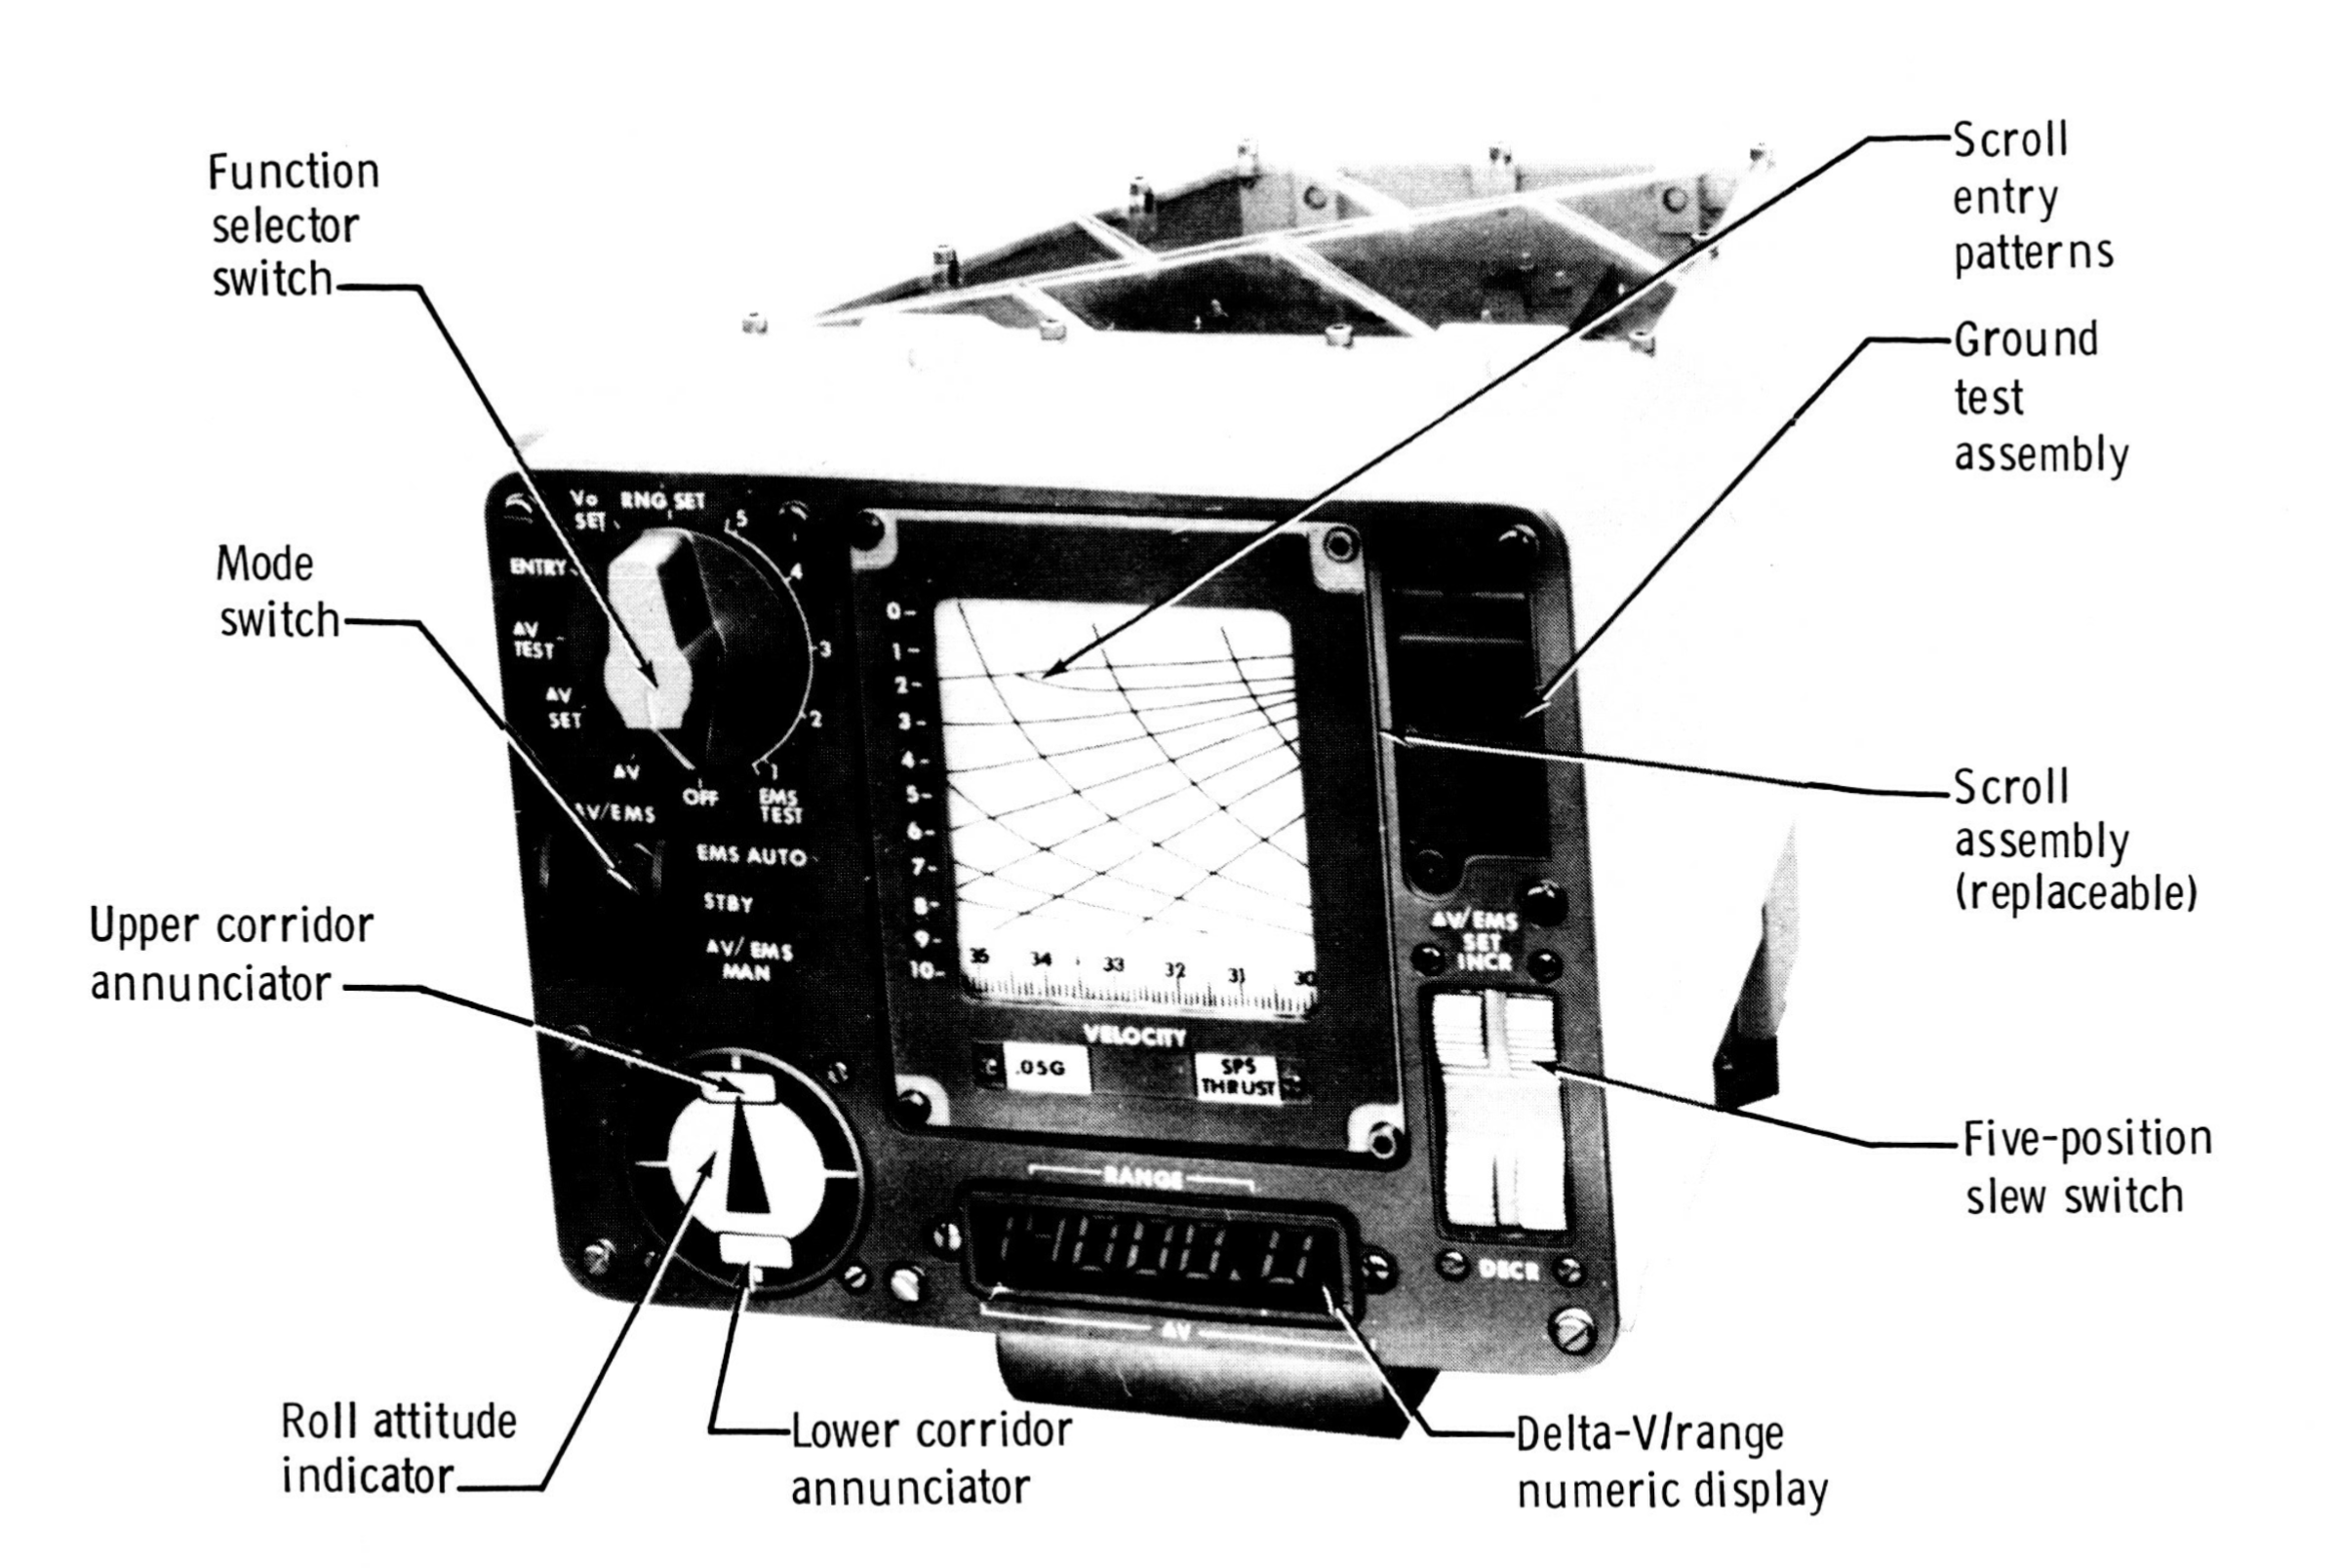
\includegraphics[width=\linewidth]{papers/leo/Grafiken/EMS.png}
	\caption{Abbildung eines EMS der Apollo-Mision, aus einem Erfahrungsbericht\,\cite{wilson1976apollo}.}
	\label{fig:leo:ems}
\end{figure}


\subsection{Warum \(\Delta V\) in der Raumfahrt so wichtig ist}
In der Raumfahrt dreht sich alles um die Anpassung der Geschwindigkeit. 
Das Ziel eines jeden Raumfluges ist es, die notwendige \(\Delta V\) zu erreichen, um von einer Phase in die nächste zu wechseln. 
Beim Aufstieg in die Erdumlaufbahn muss die Rakete eine bestimmte \(\Delta V\) aufbringen, um die Orbitalgeschwindigkeit zu erreichen. 
Beim Wechsel in eine Transferbahn, wie zum Beispiel zum Mond, wird erneut \(\Delta V\) benötigt, um die erforderliche Fluggeschwindigkeit für die Transferphase zu erreichen.

Der Grund für die Fixierung der Raketentechniker auf Geschwindigkeit ist klar: Ohne die richtige Geschwindigkeit stürzt die Rakete zur Erde zurück. 
Mit der richtigen \(\Delta V\) jedoch bleibt sie in der Umlaufbahn. Daher spielt die Diskussion über Geschwindigkeitsverluste und die optimale Steuerung eine entscheidende Rolle bei der Missionsplanung.

